\appendix{Представление графического материала}

Графический материал, выполненный на отдельных листах,
изображен на рисунках А.1--А.\arabic{числоПлакатов}.
\setcounter{числоПлакатов}{0}

\renewcommand{\thefigure}{А.\arabic{figure}} % шаблон номера для плакатов

\begin{landscape}

\begin{плакат}
    
\includegraphics[width=0.82\linewidth]{титульник.eps}
    \заголовок{Сведения о ВКРБ}
    \label{pl1:image}      
\end{плакат}

\begin{плакат}
	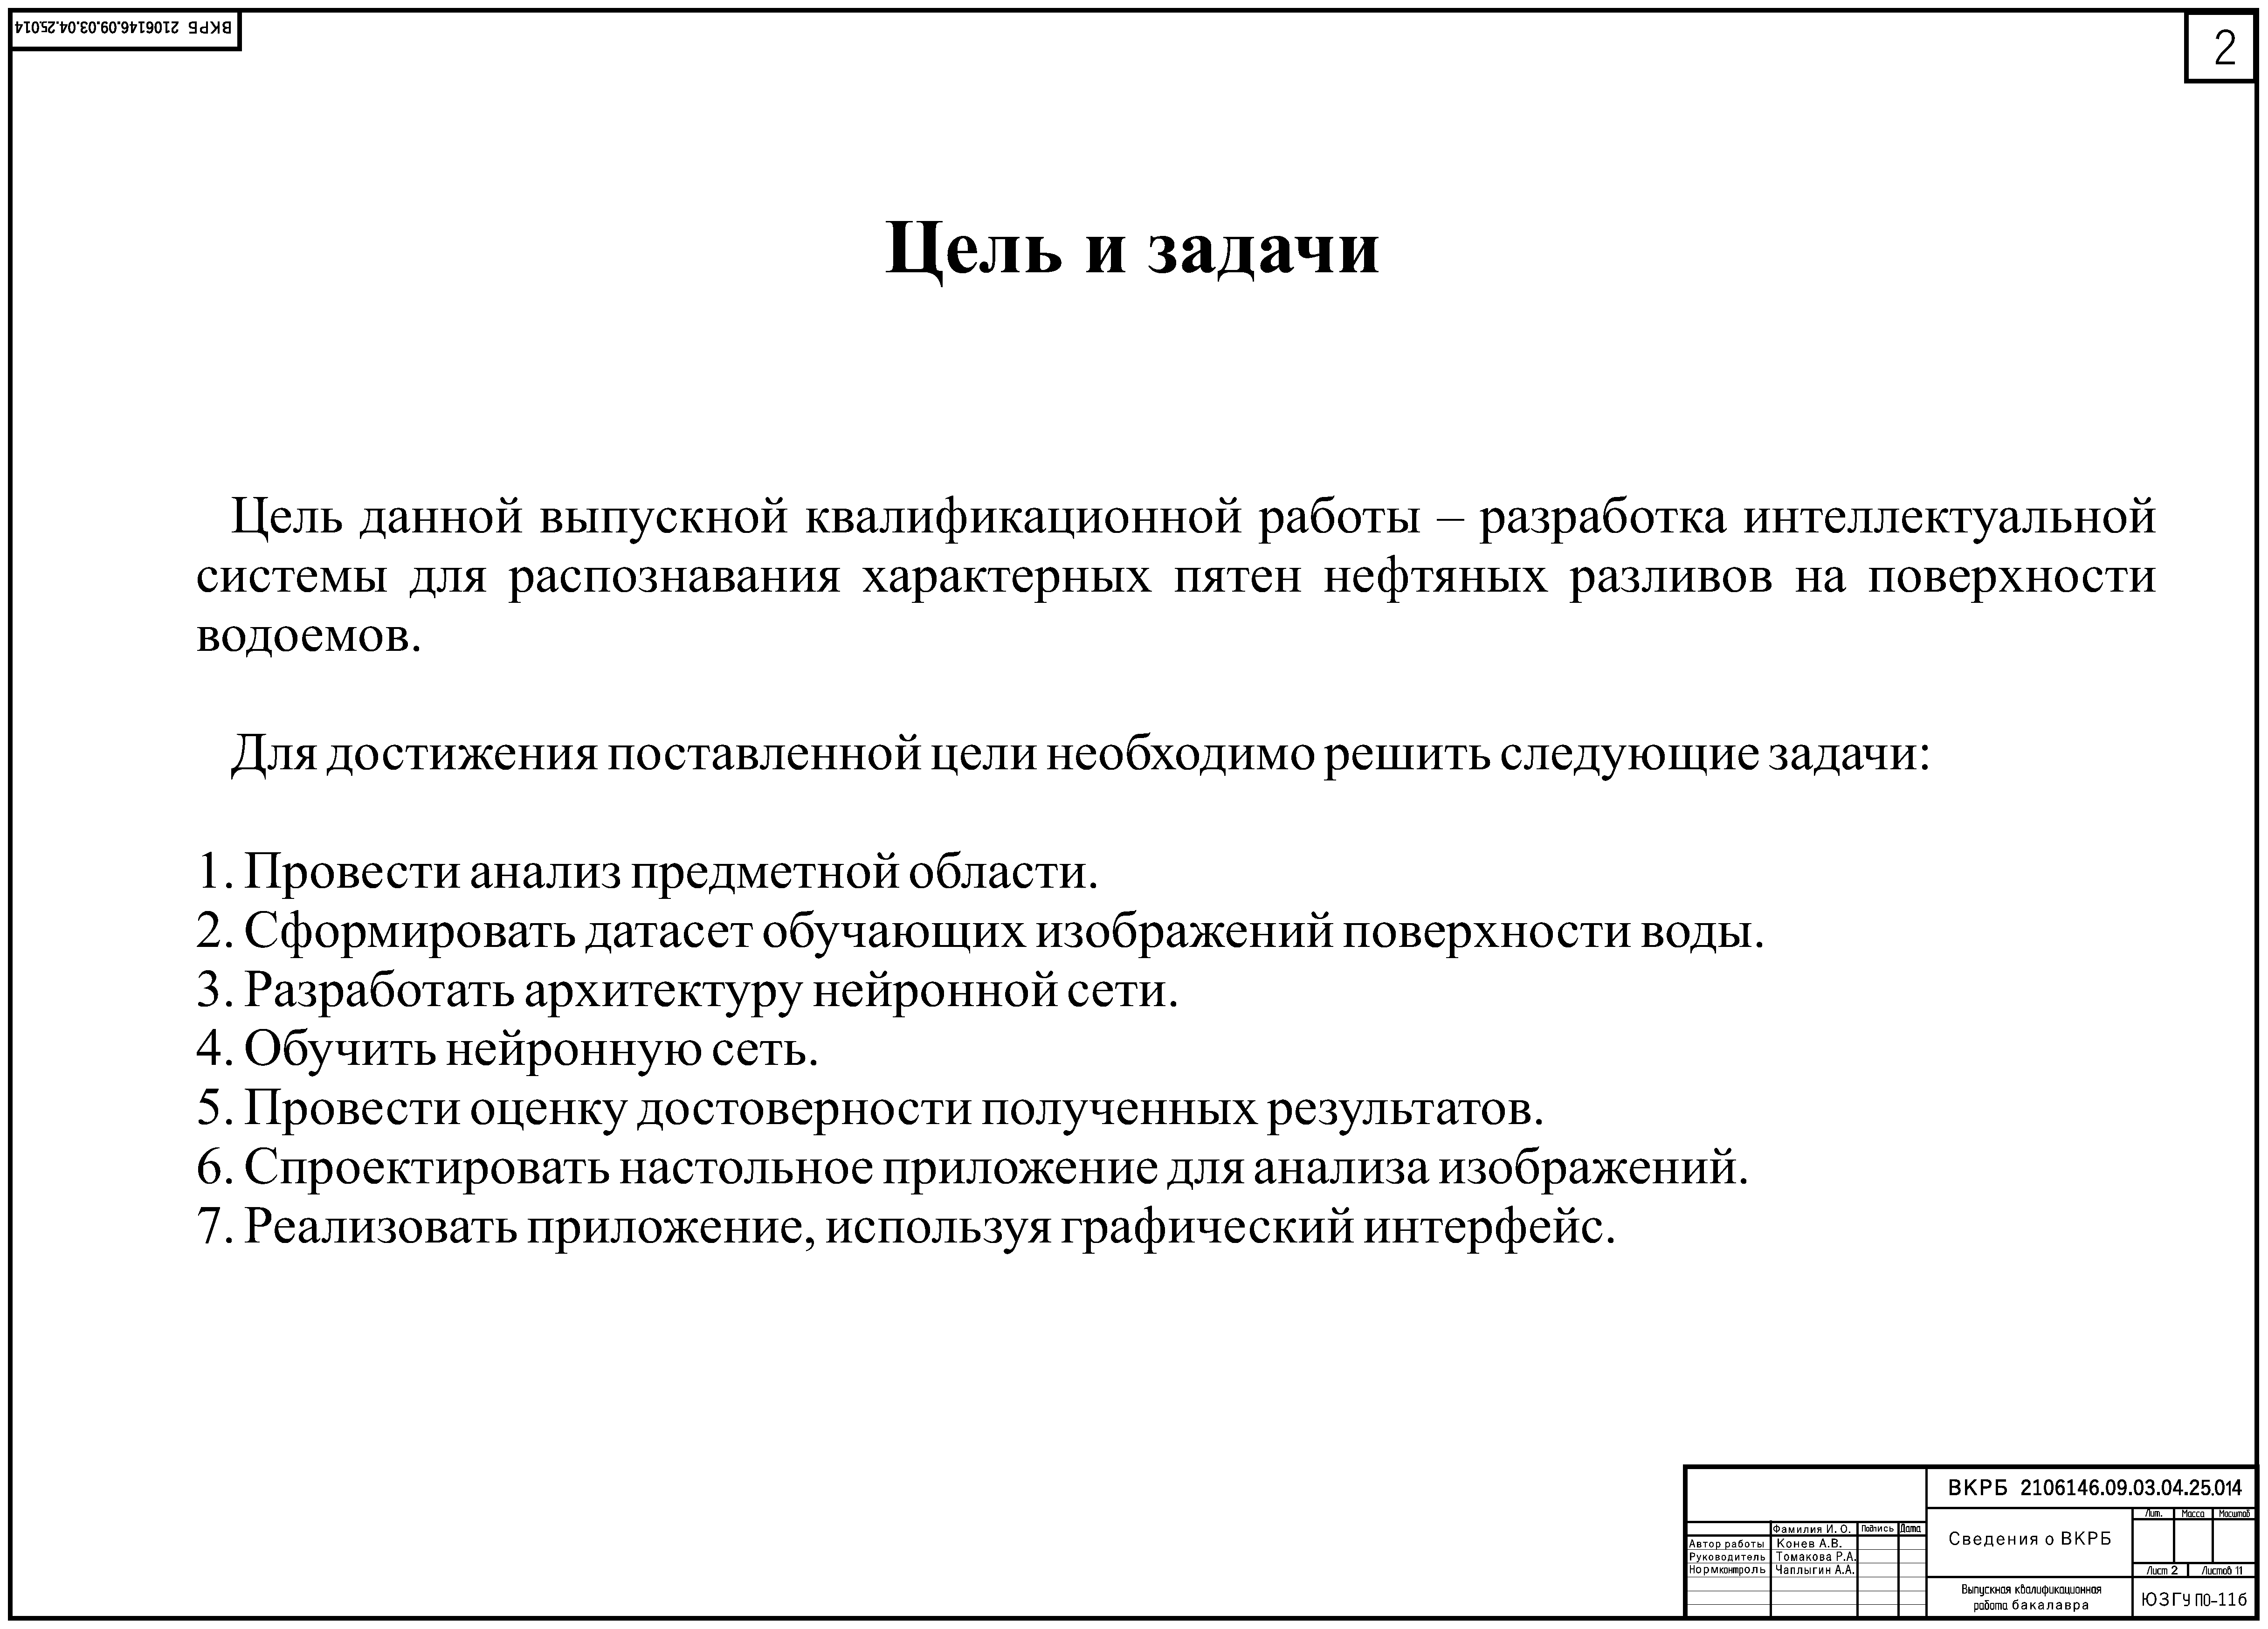
\includegraphics[width=0.82\linewidth]{цель и задачи.eps}
	\заголовок{Цель и задачи работы}
	\label{pl2:image}      
\end{плакат}

\begin{плакат}
	
\includegraphics[width=0.82\linewidth]{диаграмма прецедентов.eps}
	\заголовок{Диаграмма прецедентов}
	\label{pl3:image}      
\end{плакат}

\begin{плакат}
	
\includegraphics[width=0.82\linewidth]{архитектура системы.eps}
	\заголовок{Архитектура интеллектуальной системы}
	\label{pl4:image}      
\end{плакат}

\begin{плакат}
	
\includegraphics[width=0.82\linewidth]{архитектура сети.eps}
	\заголовок{Архитектура нейронной сети}
	\label{pl5:image}      
\end{плакат}

\begin{плакат}
	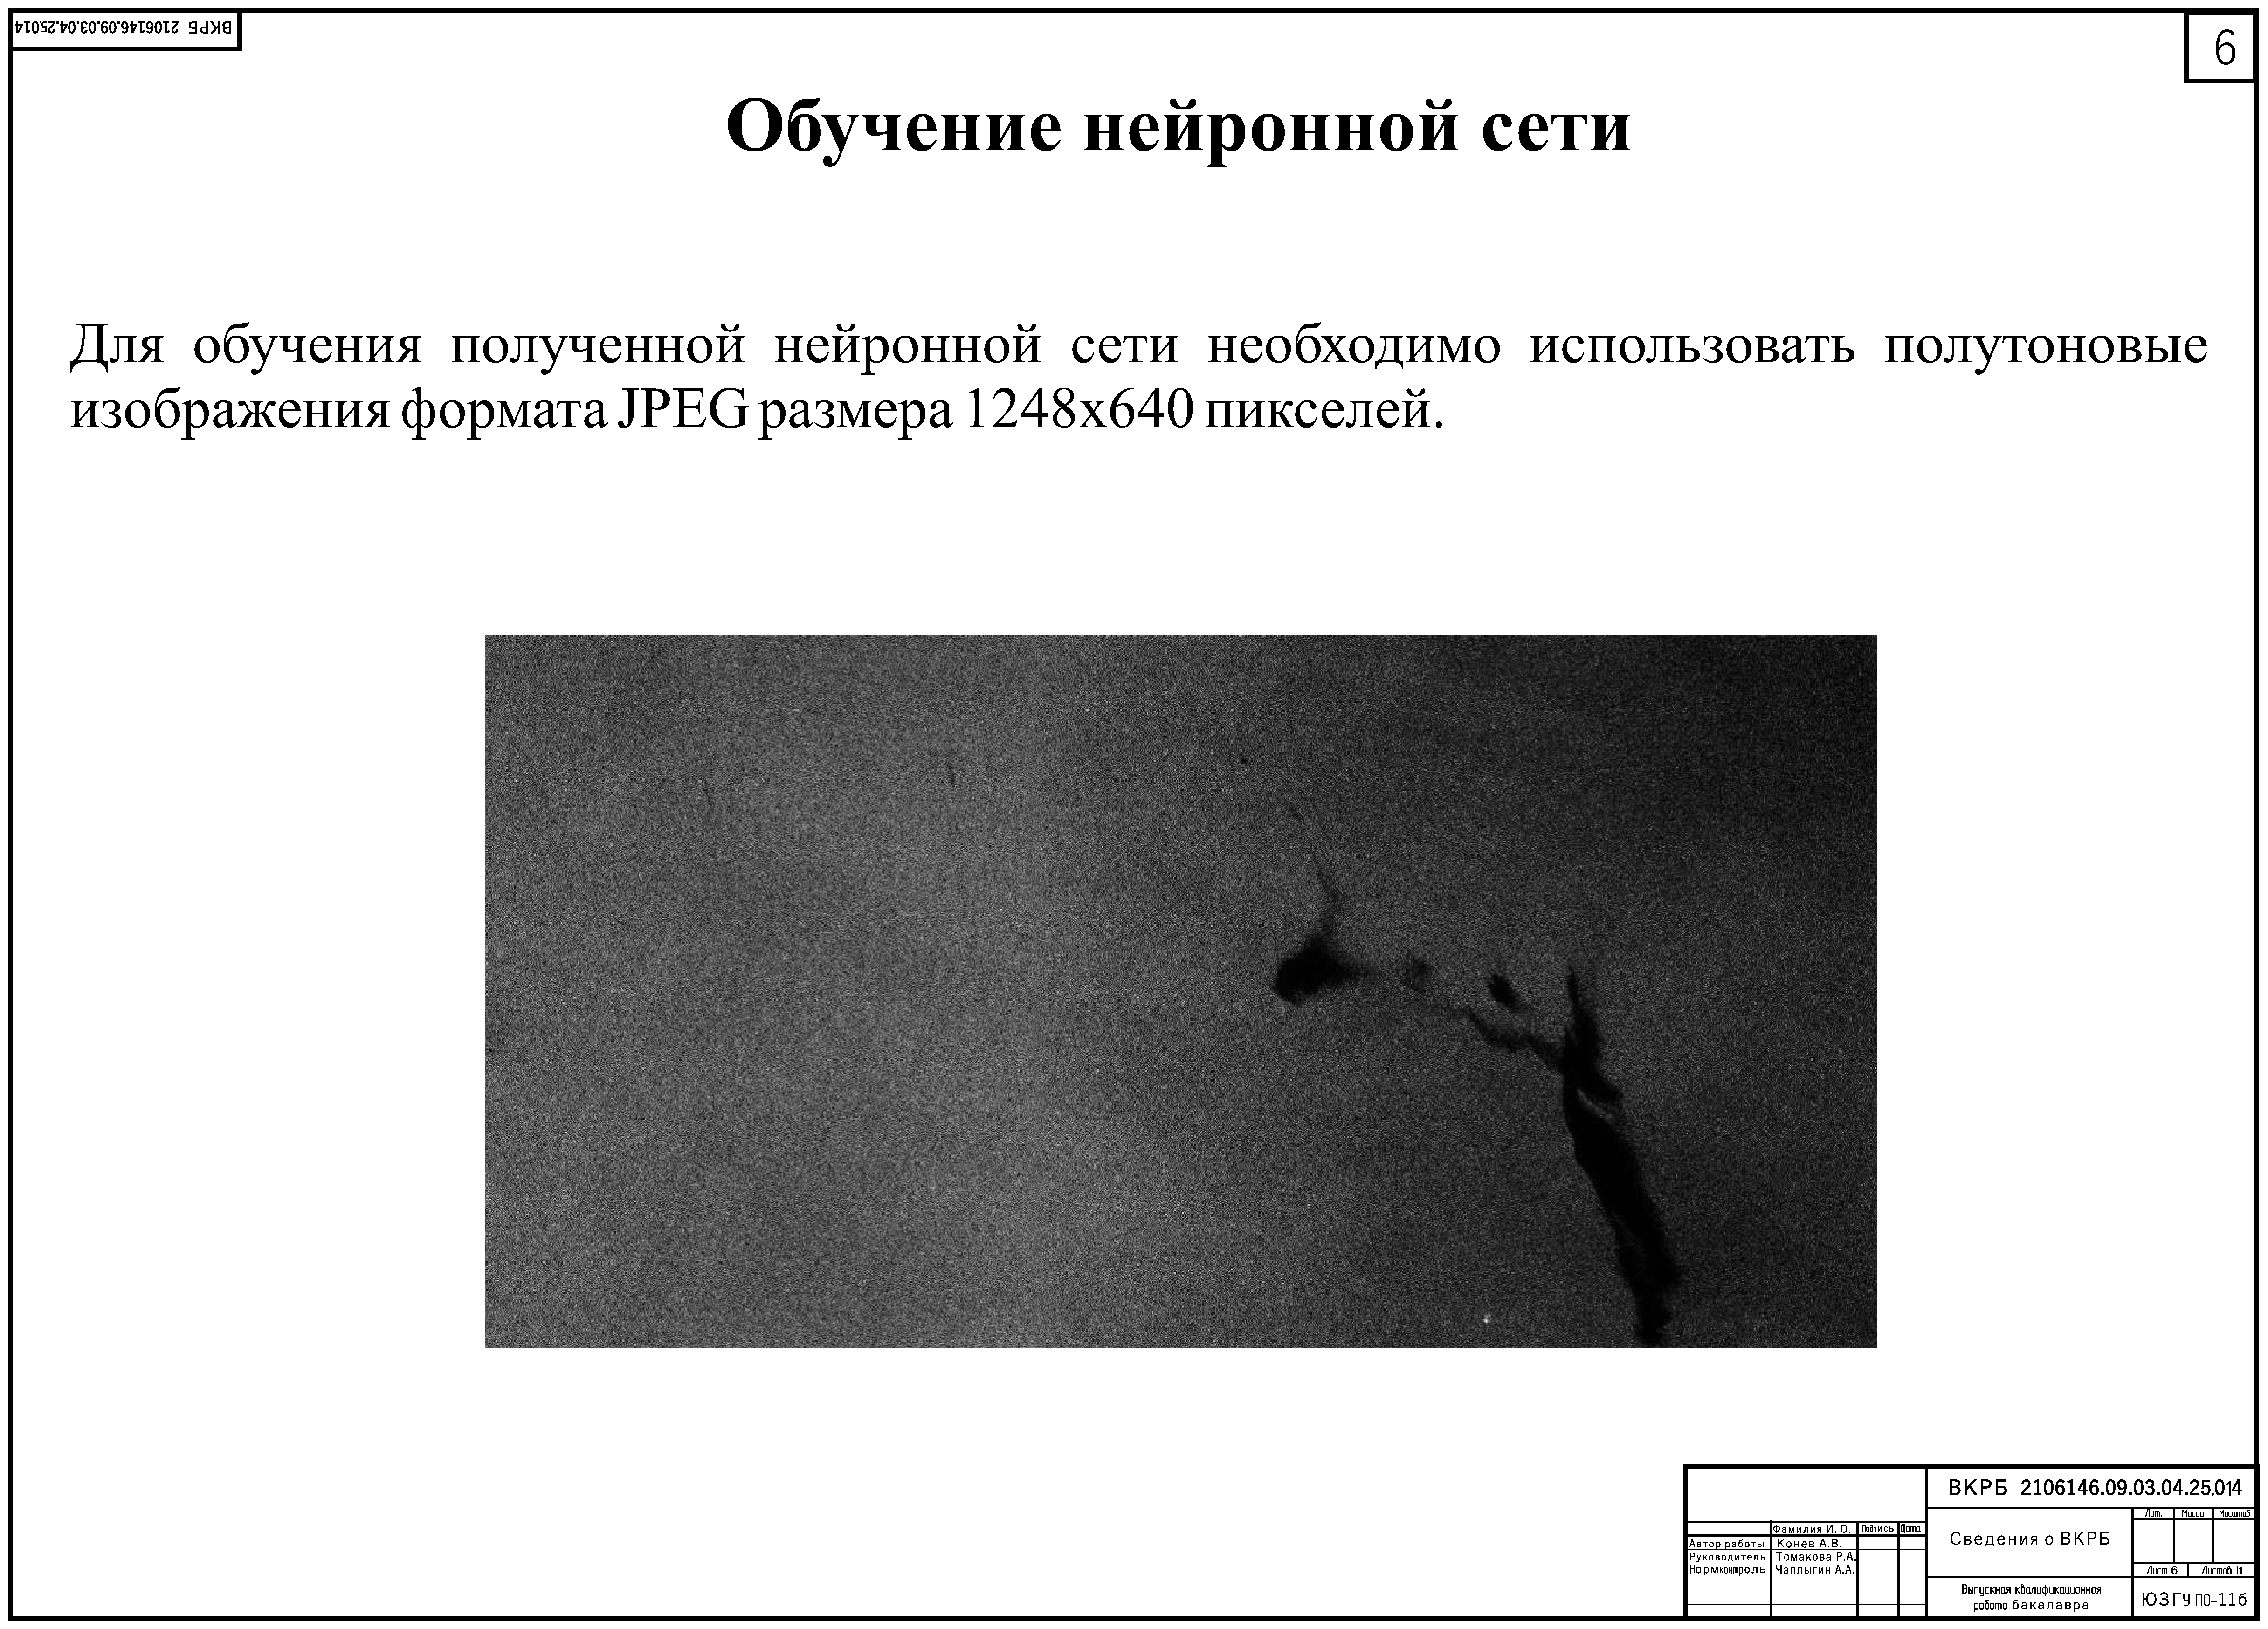
\includegraphics[width=0.82\linewidth]{обучение нейросети.eps}
	\заголовок{Обучение нейронной сети}
	\label{pl6:image}      
\end{плакат}

\begin{плакат}
	
\includegraphics[width=0.82\linewidth]{интерфейс анализ.eps}
	\заголовок{Окно анализа изображения}
	\label{pl7:image}      
\end{плакат}

\begin{плакат}
	
\includegraphics[width=0.82\linewidth]{интерфейс обучение.eps}
	\заголовок{Окно обучения нейронной сети}
	\label{pl8:image}      
\end{плакат}

\begin{плакат}
	
\includegraphics[width=0.82\linewidth]{интерфейс тестирование.eps}
	\заголовок{Окно тестирования нейронной сети}
	\label{pl9:image}      
\end{плакат}

\begin{плакат}
	
\includegraphics[width=0.82\linewidth]{результаты тестирования сети.eps}
	\заголовок{Тестирование обученной нейронной сети}
	\label{pl10:image}      
\end{плакат}

\begin{плакат}
	
\includegraphics[width=0.82\linewidth]{заключение.eps}
	\заголовок{Заключение}
	\label{pl11:image}      
\end{плакат}

\end{landscape}
